\documentclass[11pt,aspectratio=169]{beamer}

\usepackage[utf8]{inputenc}
\usepackage[T1]{fontenc}
\usepackage[spanish,es-tabla]{babel}
\usepackage{lmodern}
\usepackage[table]{xcolor}
\usepackage{booktabs}
\usepackage{tikz}
\usetikzlibrary{positioning, arrows.meta, fit, shapes.geometric, calc}
\usepackage[most]{tcolorbox}
\usepackage{microtype}
\usepackage{pifont}

\definecolor{accent}{HTML}{1F6FEB}
\definecolor{accent2}{HTML}{0A8754}
\definecolor{warn}{HTML}{D1351A}
\definecolor{bg}{HTML}{F6F8FA}
\definecolor{bgbox}{HTML}{EDF2F7}
\definecolor{rule}{HTML}{D0D7DE}
\definecolor{ink}{HTML}{1F2328}
\definecolor{muted}{HTML}{57606A}
\definecolor{good}{HTML}{1A7F37}

\usetheme{default}
\setbeamercolor{normal text}{fg=ink, bg=white}
\setbeamercolor{frametitle}{fg=accent, bg=white}
\setbeamercolor{title}{fg=ink}
\setbeamercolor{itemize item}{fg=accent}
\setbeamercolor{itemize subitem}{fg=accent}
\setbeamercolor{block title}{bg=bgbox, fg=accent}
\setbeamercolor{block body}{bg=bg, fg=ink}
\setbeamercolor{footline}{fg=muted}

\setbeamerfont{frametitle}{size=\Large, series=\bfseries}
\setbeamerfont{title}{size=\huge, series=\bfseries}

\setbeamertemplate{navigation symbols}{}
\setbeamertemplate{itemize item}{\raisebox{0.15ex}{\scriptsize\textbullet}}

\setbeamertemplate{frametitle}{%
  \nointerlineskip
  \vspace*{0.4em}
  \begin{beamercolorbox}[wd=\paperwidth, leftskip=0.6cm, rightskip=0.6cm]{frametitle}
    \insertframetitle\par
    \vspace*{0.15em}
    \textcolor{rule}{\rule{\dimexpr\paperwidth-1.2cm\relax}{0.4pt}}
  \end{beamercolorbox}
}

\setbeamertemplate{footline}{%
  \leavevmode%
  \hbox{%
    \begin{beamercolorbox}[wd=0.5\paperwidth, ht=2.5ex, dp=1ex, leftskip=0.6cm]{footline}
      \usebeamerfont{footline}\small TP3 · Perceptrones (versión resumida)
    \end{beamercolorbox}%
    \begin{beamercolorbox}[wd=0.5\paperwidth, ht=2.5ex, dp=1ex, rightskip=0.6cm]{footline}
      \hfill\usebeamerfont{footline}\small\insertframenumber\,/\,\inserttotalframenumber
    \end{beamercolorbox}%
  }%
}

\newtcolorbox{insight}{
  enhanced, breakable,
  colback=bgbox, colframe=accent,
  boxrule=0pt, leftrule=4pt,
  arc=2pt, outer arc=0pt,
  left=8pt, right=8pt, top=4pt, bottom=4pt
}
\newtcolorbox{warning}{
  enhanced, breakable,
  colback=bgbox, colframe=warn,
  boxrule=0pt, leftrule=4pt,
  arc=2pt, outer arc=0pt,
  left=8pt, right=8pt, top=4pt, bottom=4pt
}
\newtcolorbox{takeaway}{
  enhanced, breakable,
  colback=accent2!8, colframe=accent2,
  boxrule=0pt, leftrule=4pt,
  arc=2pt, outer arc=0pt,
  left=8pt, right=8pt, top=4pt, bottom=4pt
}

\newcommand{\code}[1]{\texttt{\textcolor{accent}{#1}}}
\newcommand{\file}[1]{\texttt{\small #1}}
\newcommand{\ok}{\textcolor{good}{\ding{52}}}
\newcommand{\nok}{\textcolor{warn}{\ding{56}}}

\newcommand{\sectiondivider}[2]{%
  \begingroup
  \setbeamercolor{background canvas}{bg=accent}
  \begin{frame}[plain]
    \centering
    \vspace*{2cm}
    \color{white}
    {\fontsize{14}{16}\selectfont\bfseries Bloque #1}\\[1.2em]
    {\fontsize{32}{38}\selectfont\bfseries #2}\\[1.5em]
    \textcolor{white!75}{\rule{6cm}{0.4pt}}\\
  \end{frame}
  \endgroup
}

\title{TP3 — Perceptrones}
\subtitle{Versión resumida}
\author{}
\institute{Sistemas de Inteligencia Artificial · ITBA · 1Q 2026}
\date{}

\setbeamertemplate{title page}{%
  \begin{tikzpicture}[remember picture, overlay]
    \fill[accent] (current page.north west) rectangle ($(current page.south west) + (0.5,0)$);
    \foreach \x in {0,...,28} {
      \foreach \y in {0,...,16} {
        \fill[accent!18] ($(current page.north west) + (1.0 + 0.5*\x, -0.6 - 0.5*\y)$) circle (1pt);
      }
    }
  \end{tikzpicture}
  \vspace*{1.4cm}
  \begin{flushleft}
    \hspace*{1cm}{\fontsize{40}{46}\selectfont\bfseries\color{ink}TP3}\\[0.3em]
    \hspace*{1cm}{\fontsize{30}{36}\selectfont\bfseries\color{accent}Perceptrones}\\[0.6em]
    \hspace*{1cm}{\Large\color{muted}\inserttitle\hfill}\\
    \hspace*{1cm}{\large\color{muted}\insertsubtitle}\\[1.6em]
    \hspace*{1cm}{\color{muted}\insertinstitute}\\
  \end{flushleft}
}

\begin{document}

% ============= 1. Portada =============
{
\setbeamertemplate{footline}{}
\begin{frame}[plain]
  \titlepage
\end{frame}
}

% ============= 2. Qué pide el TP =============
\begin{frame}{Qué pide el TP}
\textbf{Tres ejercicios sobre perceptrones, todos evaluados experimentalmente.}\\[0.6em]

\begin{tabular}{@{}p{0.18\linewidth}p{0.78\linewidth}@{}}
\toprule
\textbf{Ej 1} & Detección de fraude por \emph{knowledge distillation} con perceptrón simple. \\
\midrule
\textbf{Ej 2} & Clasificación de dígitos manuscritos (10 clases, 28$\times$28). \\
\midrule
\textbf{Ej 3} & Mismo problema, target: \textbf{accuracy $\geq 98\%$ en test}. \\
\bottomrule
\end{tabular}\\[1em]

\begin{warning}
\textbf{Regla de evaluación:} \code{digits\_test.csv} se evalúa \emph{una sola vez}, al final, con el config ganador congelado. No se toca durante búsqueda de hiperparámetros.
\end{warning}
\end{frame}

% ===================================================================
\sectiondivider{1 / 4}{Decisiones de diseño}

% ============= 3. Las 7 decisiones — overview =============
\begin{frame}{Siete decisiones que afectan a todos los ejercicios}
\centering\footnotesize
\begin{tabular}{@{}p{0.20\linewidth}p{0.27\linewidth}p{0.27\linewidth}p{0.20\linewidth}@{}}
\toprule
\textbf{Decisión} & \textbf{Ej 1 (perceptrón simple)} & \textbf{Ej 2 / Ej 3 (MLP)} & \textbf{Backing} \\
\midrule
1. Activación        & sigmoide (target $[0,1]$)  & ReLU + softmax salida & literatura estándar \\
\rowcolor{bgbox}
2. Inicialización    & uniform $[-0.1,+0.1]$      & \emph{auto}: He (ReLU), Xavier (softmax) & HTML cátedra \\
3. Optimizador       & SGD online                  & \textbf{Adam} (lr=$10^{-3}$) & PDF optimizadores \\
\rowcolor{bgbox}
4. Learning rate     & fijo (config)              & \textbf{$10^{-3}$} (sweep) & PDF optimizadores \\
5. Función de costo  & MSE                         & cross-entropy (multiclase) & literatura estándar \\
\rowcolor{bgbox}
6. Convergencia      & $\varepsilon$ sobre MSE de train & early stopping val\_loss (patience=10) & slide 14 PDF reg. \\
7. Bias              & bias trick (col.\ de 1's)  & bias trick + \emph{no} se penaliza con L2 & Goodfellow Cap.~7 \\
\bottomrule
\end{tabular}\\[0.6em]

\begin{insight}
\textbf{Estrategia online vs.\ mini-batch:} Ej 1 = online estricto (un update por muestra, regla del apunte). Ej 2 / Ej 3 = mini-batch con \textbf{B=16} (elegido por sweep, mejor val\_acc + más rápido).
\end{insight}
\end{frame}

% ============= 4. Validación experimental =============
\begin{frame}{Las elecciones críticas se validaron con sweep (Ej 2)}
\small\textbf{Coarse-to-fine:} Fase 1 (k-fold=1, exploratoria) $\to$ \code{base.json} $\to$ Fase 2 (k-fold=5, validación).\\[0.6em]

\centering\footnotesize
\begin{tabular}{@{}p{0.18\linewidth}p{0.42\linewidth}p{0.34\linewidth}@{}}
\toprule
\textbf{HP} & \textbf{Ganador} & \textbf{Comentario} \\
\midrule
Optimizador  & \textbf{Adam} (96.74\%) & Momentum 96.34\%, SGD 94.81\% (no convergió). \\
\rowcolor{bgbox}
LR           & \textbf{$10^{-3}$} (96.74\%) & $10^{-4}$ lento; $\geq 10^{-2}$ overshooting; $0.1$ y $10$ diverge. \\
Arquitectura & $[784,100,50,10]$ (96.22\%) & Empate técnico con \code{wider} \([200,100]\); elegida por \textbf{parsimonia}. \\
\rowcolor{bgbox}
Init         & empate técnico ($\sim 96\%$) & He / Xavier / Uniform iguales (std $\sim 0.3\%$). \\
Activación   & ReLU (96.22\%) & Sigmoid 96.01\%, tanh 95.94\%; ReLU converge $\sim 3\times$ más rápido. \\
\rowcolor{bgbox}
Batch        & \textbf{16} (mejor macro\_F1) & 32/64/128 empatan en val\_acc, $\geq 7$ epochs vs.\ 3. \\
\bottomrule
\end{tabular}\\[0.6em]

\begin{takeaway}
\textbf{Solo el sweep de LR mostró rangos catastróficos.} Las demás dimensiones rinden parecido $\Rightarrow$ elegimos por \textbf{parsimonia} (más simple / más rápido a igual rendimiento).
\end{takeaway}
\end{frame}

% ===================================================================
\sectiondivider{2 / 4}{Ej 1 — Detección de fraude}

% ============= 5. Ej1 — Setup =============
\begin{frame}{Ej 1 — El problema}
\textbf{Knowledge distillation:} replicar la salida del BigModel (probabilidad de fraude) con un TinyModel (perceptrón simple).\\[0.6em]

\begin{columns}[T]
\column{0.55\linewidth}
\textbf{Datos:} \file{fraud\_dataset.csv} (9 features, $\sim 50$k filas).\\[0.4em]

\textbf{Target de entrenamiento:}\\
\code{big\_model\_fraud\_probability} (continuo en $[0,1]$).\\[0.4em]

\textbf{Ground truth (eval):}\\
\code{flagged\_fraud} (binaria 0/1).

\column{0.45\linewidth}
\begin{warning}
\textbf{Regla del enunciado:}\\ \code{flagged\_fraud} \emph{nunca} se usa para entrenar.
\end{warning}
\vspace{0.6em}

\textbf{Salida esperada en $[0,1]$} $\Rightarrow$ activación sigmoide en TinyModel.
\end{columns}
\end{frame}

% ============= 6. Ej1 — Lineal vs No-Lineal =============
\begin{frame}{Ej 1 — Lineal vs No-Lineal: la sigmoide gana claro}
\centering
\begin{tabular}{@{}lr@{}}
\toprule
\textbf{Modelo} & \textbf{MSE test (mean $\pm$ std)} \\
\midrule
Lineal (Adaline)        & $0.0266 \pm 0.0008$ \\
\rowcolor{accent2!15}
\textbf{No-Lineal (sigmoide)} & $\boldsymbol{0.0110 \pm 0.0004}$ \quad ($\boldsymbol{-59\%}$) \\
\bottomrule
\end{tabular}\\[1em]

\begin{insight}
El target es una probabilidad acotada en $[0,1]$. La sigmoide \emph{naturalmente} mapea su salida a ese rango; el lineal puede producir valores fuera de $[0,1]$ y el MSE penaliza fuerte esa salida fuera de dominio.
\end{insight}
\end{frame}

% ============= 7. Ej1 — Threshold y recomendación =============
\begin{frame}{Ej 1 — Threshold óptimo y recomendación}
\textbf{Threshold default 0.5 luce terrible} (precision 0.333, recall 1.000). No es el modelo: las salidas sigmoide se concentran en la parte alta (mediana de scores: 0.99).\\[0.6em]

\centering\small
\begin{tabular}{@{}lcccl@{}}
\toprule
\textbf{Threshold} & \textbf{Precision} & \textbf{Recall} & \textbf{F1} & \textbf{Caso de uso} \\
\midrule
0.50 (default)     & 0.333 & 1.000 & 0.499 & --- \\
\rowcolor{accent2!15}
\textbf{0.89} (óptimo F1) & \textbf{0.886} & \textbf{0.861} & \textbf{0.873} & auditoría manual barata \\
0.95               & 0.949 & 0.746 & 0.835 & FP costosos \\
0.99               & 1.000 & 0.527 & 0.690 & cero tolerancia a FP \\
\bottomrule
\end{tabular}\\[0.6em]

\textcolor{muted}{\footnotesize AUC-ROC = 0.9921 (lineal: 0.9720) — capacidad de \emph{ranking} excelente.}\\[0.4em]

\begin{takeaway}
\textbf{El modelo entrega scores; la política de threshold es decisión de negocio.} Recomendación: $0.89$ si los falsos positivos son baratos; $\geq 0.95$ si son costosos.
\end{takeaway}
\end{frame}

% ===================================================================
\sectiondivider{3 / 4}{Ej 2 — Clasificación de dígitos}

% ============= 8. Ej2 — Problema =============
\begin{frame}{Ej 2 — El problema y la arquitectura final}
\begin{columns}[T]
\column{0.5\linewidth}
\textbf{Datos:}
\begin{itemize}
  \item Train: \file{digits.csv} (12.449 muestras)
  \item Test: \file{digits\_test.csv} (2.498)
\end{itemize}
Cada muestra: vector 784 floats $\in [0,1]$ (28$\times$28 flatten), label 0--9.

\column{0.5\linewidth}
\textbf{Arquitectura final:}
\begin{itemize}
  \item Input: 784
  \item Hidden 1: 100 (ReLU)
  \item Hidden 2: 50 (ReLU)
  \item Output: 10 (Softmax)
\end{itemize}
Loss: cross-entropy. Adam ($lr=10^{-3}$). Batch=16. Early stopping (patience=10).
\end{columns}
\vspace{0.6em}

\begin{warning}
\textbf{Regla:} \code{digits\_test.csv} se evalúa \textbf{una sola vez} al final.
\end{warning}
\end{frame}

% ============= 9. Ej2 — Experimentación =============
\begin{frame}{Ej 2 — La experimentación, en una slide}
\centering
\begin{tikzpicture}[
  every node/.style={font=\small},
  phase/.style={
    draw=accent, fill=bg, rounded corners=3pt,
    minimum width=3.6cm, minimum height=1.5cm, align=center
  },
  result/.style={
    draw=accent2, fill=accent2!10, rounded corners=3pt,
    minimum width=3.6cm, minimum height=1.5cm, align=center
  },
  arrow/.style={-{Latex[length=3mm]}, accent, very thick}
]
  \node[phase] (f1) {\textbf{Fase 1} (k=1)\\\footnotesize sweeps secuenciales\\\footnotesize arch \(\to\) opt \(\to\) LR \(\to\) batch};
  \node[result, right=1.4cm of f1] (base) {\textbf{base.json}\\\footnotesize ganador\\\footnotesize consolidado};
  \node[phase, right=1.4cm of base] (f2) {\textbf{Fase 2} (k=5)\\\footnotesize one-at-a-time\\\footnotesize valida con K-fold};
  \node[result, below=0.7cm of base] (final) {\textbf{final\_eval}\\\footnotesize digits\_test.csv\\\footnotesize (UNA sola vez)};

  \draw[arrow] (f1) -- (base);
  \draw[arrow] (base) -- (f2);
  \draw[arrow] (f2.south) -- ++(0,-0.4) -| (final.east);
  \draw[arrow, dashed] (base.south) -- (final.north);
\end{tikzpicture}\\[0.6em]

\begin{insight}
\textbf{Coarse-to-fine}: Fase 1 reduce el espacio de búsqueda con sweeps rápidos. Fase 2 valida con K-fold=5. \\
$\Rightarrow$ La metodología de Fase 1 ya hace el grueso; Fase 2 confirma que las elecciones son robustas, no suerte de un solo split.
\end{insight}
\end{frame}

% ============= 10. Ej2 — Resultados val + final eval =============
\begin{frame}{Ej 2 — Resultados: val K-fold vs.\ test (el cachetazo)}
\centering\Large
val K-fold=5: \textbf{96.22\% $\pm$ 0.43\%}\\[0.4em]
\textcolor{muted}{$\downarrow$ \footnotesize (final\_eval contra digits\_test.csv, UNA sola vez)}\\[0.4em]
test: \textcolor{warn}{\textbf{86.30\%}}\\[0.6em]
\Large \textbf{Drop de 10 puntos porcentuales.}\\[0.8em]

\normalsize
\begin{warning}
\textbf{Distribution shift, no underfitting.} El modelo está bien — los datos no se parecen. Diez veces más grande que el std del K-fold (0.43\%). Imposible que sea ruido.
\end{warning}
\end{frame}

% ============= 11. Ej2 — Análisis matriz =============
\begin{frame}{Ej 2 — La matriz de confusión confirma el shift}
\begin{columns}[T]
\column{0.5\linewidth}
\centering
\textbf{Val K-fold (digits.csv)}\\[0.3em]
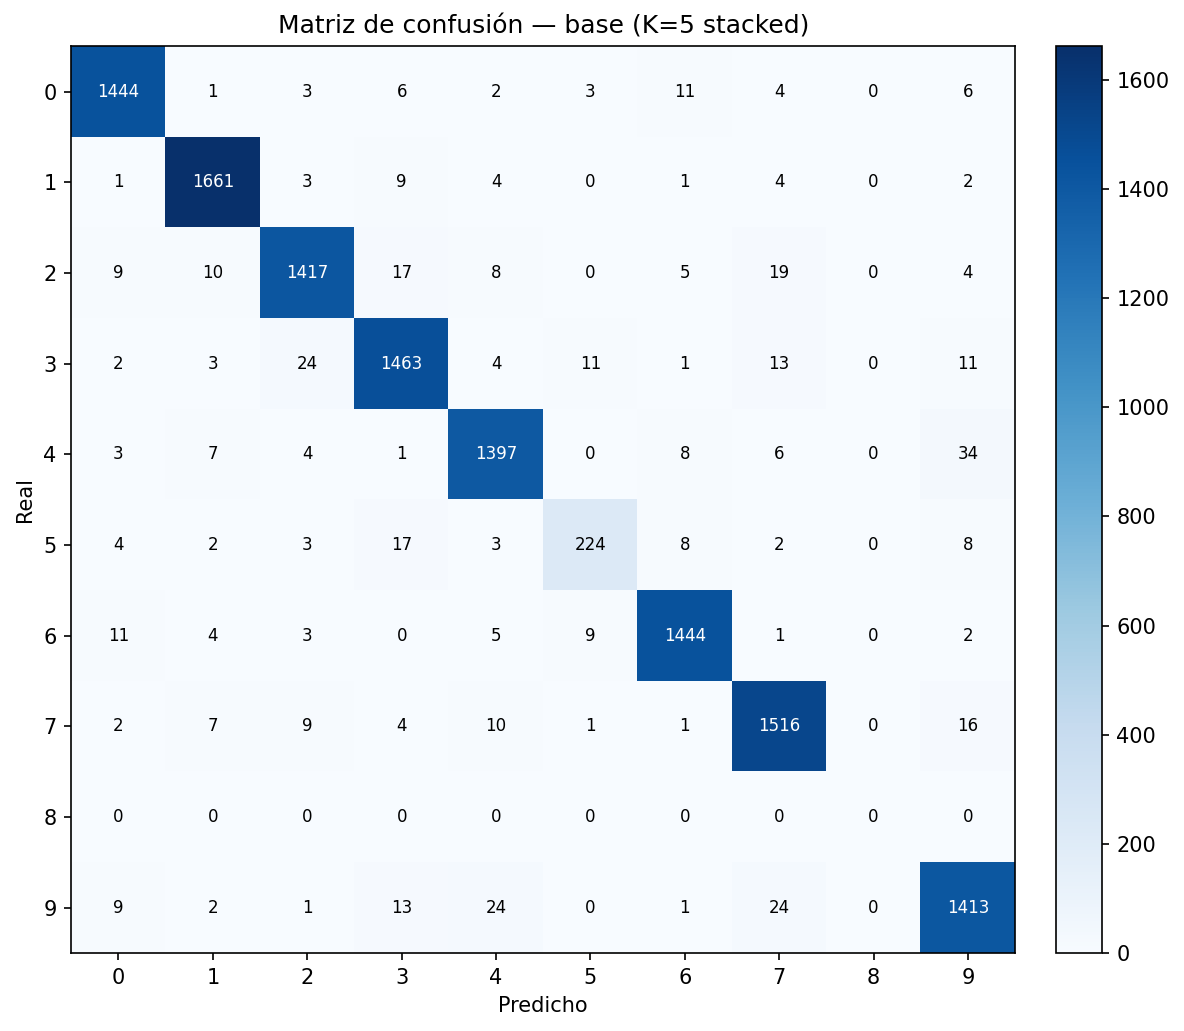
\includegraphics[width=0.8\linewidth]{../../ejercicio2/presentacion/04_confusion_matrix_base.png}\\
\textcolor{muted}{\footnotesize Diagonal limpia para 9 clases. Clase 8 colapsa.}

\column{0.5\linewidth}
\centering
\textbf{Test (digits\_test.csv)}\\[0.3em]
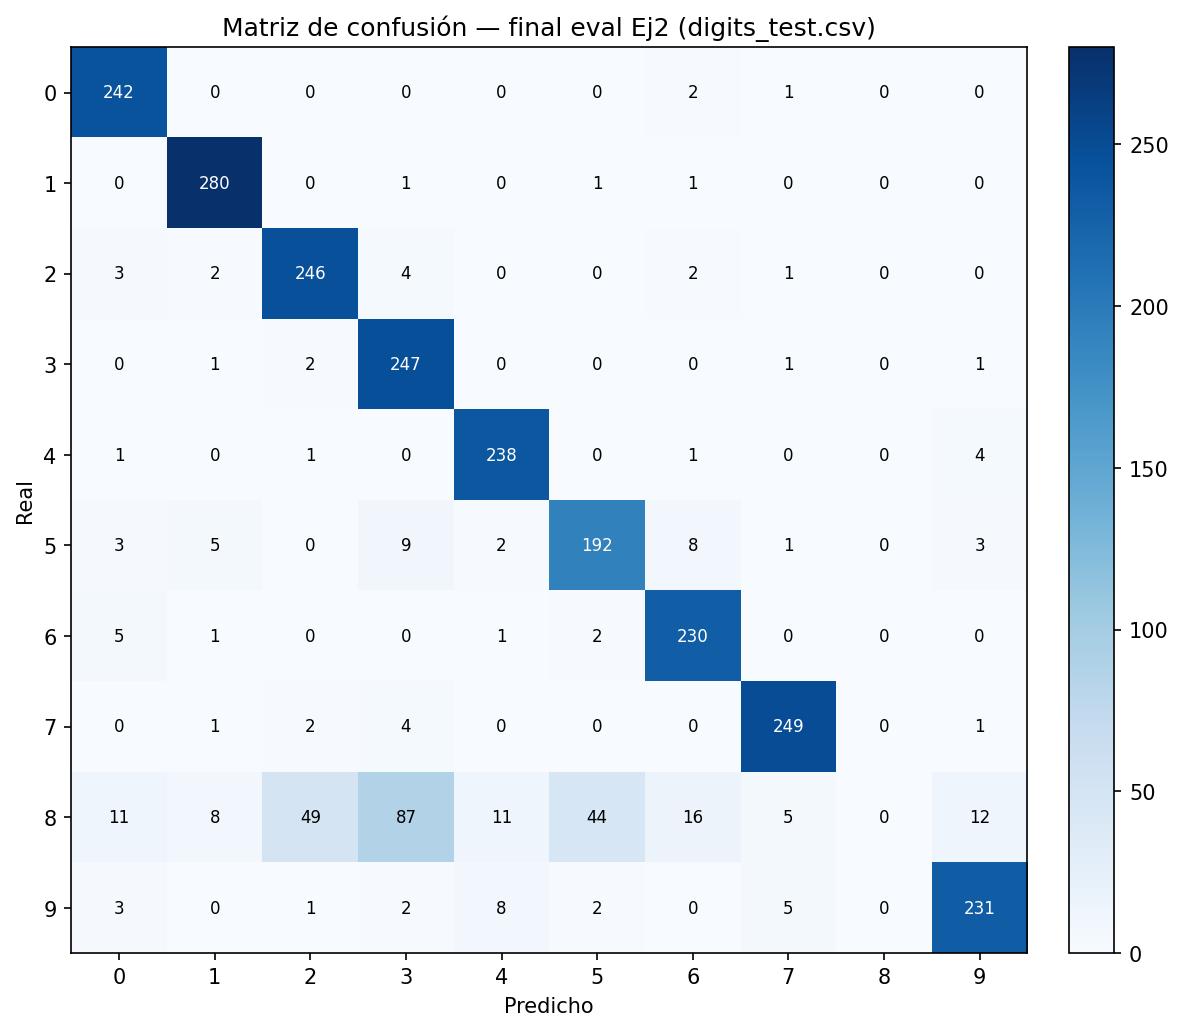
\includegraphics[width=0.8\linewidth]{../../ejercicio2/presentacion/08_confusion_matrix_final.png}\\
\textcolor{muted}{\footnotesize Confusiones distribuidas en todo el grid.}
\end{columns}
\vspace{0.6em}

\begin{takeaway}
\textbf{No es falta de capacidad ni una clase específica que falla.} Es shift entre las distribuciones de \code{digits.csv} y \code{digits\_test.csv} $\Rightarrow$ \textbf{más datos}, no más modelo.
\end{takeaway}
\end{frame}

% ===================================================================
\sectiondivider{4 / 4}{Ej 3 — Mejorar el accuracy}

% ============= 12. Ej3 — Plan + dominó =============
\begin{frame}{Ej 3 — Plan y el primer dominó: más datos}
\textbf{Hipótesis:} el techo del Ej 2 es por shift, no falta de capacidad. \\
\textbf{Plan secuencial:} (1) más datos $\to$ (2) Pack C (regularización) $\to$ (3) capacidad si nada llega.\\[0.6em]

\centering\Huge
val K=5: $96.22\% \to 97.06\%$\\[0.3em]
test: \textcolor{warn}{$86.30\%$} $\to$ \textcolor{accent2}{$\boldsymbol{96.36\%}$}\\[0.6em]
\Large\textbf{+10 puntos porcentuales en test.}\\
\large\textbf{\textcolor{muted}{Cero cambios al modelo. Solo \code{more\_digits.csv} (15.742 muestras extras).}}\\[0.8em]

\normalsize
\begin{takeaway}
\textbf{Macro F1: $0.857 \to 0.959$.} La clase 8, que estaba colapsada en Ej 2, ahora se predice correctamente. \\
$\Rightarrow$ Hipótesis del shift confirmada. Pero faltan $\sim 1.6$ pp para llegar al 98\%.
\end{takeaway}
\end{frame}

% ============= 13. Ej3 — Pack C ↔ clase de regularización =============
\begin{frame}{Ej 3 — Pack C $\leftrightarrow$ clase de regularización}
\small ¿Qué dice el PDF de regularización y qué implementamos?\\[0.3em]

\centering\footnotesize
\begin{tabular}{@{}p{0.50\linewidth}cp{0.36\linewidth}@{}}
\toprule
\textbf{Técnica del PDF} & \textbf{Impl.} & \textbf{Resultado en Ej 3} \\
\midrule
Early stopping (slide 14)                       & \ok & Activo en todos los configs \\
\rowcolor{accent2!10}
\textbf{Augmentation gaussiano} (slide 18)      & \ok & $\sigma=0.05$, $+0.32$ pp (parte del ganador) \\
Augmentation rotaciones / traslaciones / escalas (slide 18) & \nok & --- \\
\rowcolor{accent2!10}
\textbf{L2 / Weight Decay} (slides 20--25)      & \ok & $\lambda = 10^{-4}$, $+0.20$ pp \\
Dropout (slide 26 — mención)                    & \ok & val sí, test no ($-0.08$ pp) \\
Modelos de ensamble / semi-supervisado / adversarial & --- & fuera de alcance \\
\bottomrule
\end{tabular}\\[0.6em]

\begin{insight}
\textbf{Lo que faltó:} las tres formas de augmentation \emph{geométrica} (rotaciones, traslaciones, escalas). Es la hipótesis principal del techo en 96.88\%.
\end{insight}
\end{frame}

% ============= 14. Ej3 — Tabla resultados =============
\begin{frame}{Ej 3 — Resultados Pack C: el ganador}
\centering\small
\begin{tabular}{@{}lrrr@{}}
\toprule
\textbf{Config} & \textbf{val K=5} & \textbf{test} & \textbf{$\Delta$ vs base\_extra} \\
\midrule
base\_extra\_data            & 0.9706 & 0.9636 & --- (referencia) \\
\quad +\,L2 (1e-4)            & 0.9758 & 0.9656 & $+0.20$ pp \\
\quad +\,dropout (p=0.2)      & 0.9750 & 0.9628 & $-0.08$ pp \\
\rowcolor{accent2!15}
\textbf{\quad +\,L2 + aug ($\sigma=0.05$)} & \textbf{0.9760} & \textbf{0.9688} & \(\boldsymbol{+0.52}\)\textbf{ pp} \\
\quad +\,L2 + aug + dropout   & 0.9768 & 0.9656 & $+0.20$ pp \\
\quad +\,wider + L2 + aug     & 0.9777 & 0.9640 & $+0.04$ pp \\
\bottomrule
\end{tabular}\\[0.6em]

\begin{takeaway}
\textbf{Ganador:} L2 + augmentation gaussiana ($\sigma=0.05$) $\to$ \textbf{96.88\% en test}.\\[0.2em]
\textbf{Dropout no transfirió}: gana en val, pierde en test (regulariza dentro de la distribución del train, no compensa el shift). \textbf{Wider mejora val, empeora test} $\Rightarrow$ descarta falta de capacidad.
\end{takeaway}
\end{frame}

% ============= 15. Ej3 — Por qué no 98 =============
\begin{frame}{Ej 3 — Por qué no llegamos al 98\%}
\centering
\Large \textcolor{warn}{\textbf{Mejor: 96.88\%. Faltan 1.12 pp.}}\\[0.6em]

\normalsize\raggedright
\textbf{Tres hipótesis ordenadas por probabilidad:}
\begin{enumerate}\setlength\itemsep{0.2em}
  \item \textbf{Augmentation insuficiente.} Gaussian noise es \emph{isotrópico} (por píxel). El shift parece ser \emph{geométrico}: rotación, traslación, grosor de trazo. Pide augmentation \textbf{geométrica}, que el slide 18 del PDF lista pero \textbf{no implementamos}.
  \item \textbf{Sub-representación en val interno del final\_eval.} Val 10\% random para early stopping puede no incluir los digits difíciles del test.
  \item \textbf{Capacidad}: improbable, \code{wider} sobreajustó (consistente con la curva U del slide 9 PDF regularización: más capacidad sin más datos $\Rightarrow$ overfitting).
\end{enumerate}
\vspace{0.4em}

\begin{takeaway}
\textbf{Próximo paso natural:} augmentation por rotación / traslación pequeñas. No implementada en este TP.
\end{takeaway}
\end{frame}

% ===================================================================
% ============= 16. Conclusiones =============
\begin{frame}{Conclusiones}
\textbf{Tres ideas para llevarse:}\\[0.4em]

\begin{enumerate}\setlength\itemsep{0.3em}
  \item \textbf{Una buena pipeline gana más que tunear hiperparámetros.}\\
        El \(+10\)\,pp del Ej 3 vino de \emph{datos}, no de modelo. La regularización aportó solo \(+0.5\)\,pp adicional.
  \item \textbf{Los empates técnicos son más comunes que los wins claros.}\\
        Mayoría de los sweeps con margen $<0.3$ pp y std $\sim 0.4\%$. Hay que elegir por \textbf{parsimonia}, no por 0.05 pp en val.
  \item \textbf{``Mejor en val'' $\neq$ ``mejor en test'' cuando hay shift.}\\
        Dropout fue el ejemplo de manual: ganador en val, perdedor en test.
\end{enumerate}
\vspace{0.4em}

\centering\small
\begin{tabular}{@{}lc@{}}
\toprule
\textbf{Item} & \textbf{Status} \\
\midrule
Ej 1 — Knowledge distillation + threshold sweep              & \ok \\
Ej 2 — sweeps + final\_eval + análisis del shift             & \ok \\
Ej 3 — \code{more\_digits.csv} + Pack C + análisis             & \ok \\
\textbf{Ej 3 — target $\geq 98\%$}                          & \nok\ \textbf{(96.88\%)} \\
\bottomrule
\end{tabular}
\end{frame}

% ============= Cierre =============
{
\setbeamercolor{background canvas}{bg=accent}
\begin{frame}[plain]
\centering
\vspace*{2cm}
\color{white}
{\fontsize{36}{42}\selectfont\bfseries Gracias.}\\[1.5em]
{\Large Preguntas.}\\[2.5em]

\textcolor{white!75}{\rule{6cm}{0.4pt}}
\end{frame}
}

\end{document}
